\subsection{Acoustic Requirements}
The Sam Mk I is a twin engine-jet airplane with a maximum takeoff weight greater than 121,254 pounds. Due to this, the Sam Mk I must comply with Chapter 14, Paragraph 14.4, Maximum Noise Levels of ICAO Annex 16, Volume I, Amendment 11-B acoustic requirements \cite{noise_14}. Chapter 14 sets maximum noise limits as a direct function of Maximum Take-off Mass in order to incorporate heavier, and louder airplanes \cite{noise_14}. There are three different positions of measuring points for aircraft noise certification: approach, lateral, and takeoff. In Chapter 14, all three points are then added up to create a cumulative effective perceived noise in decibels (EPNdB) value.    



\begin{figure}[H]
    \centering
    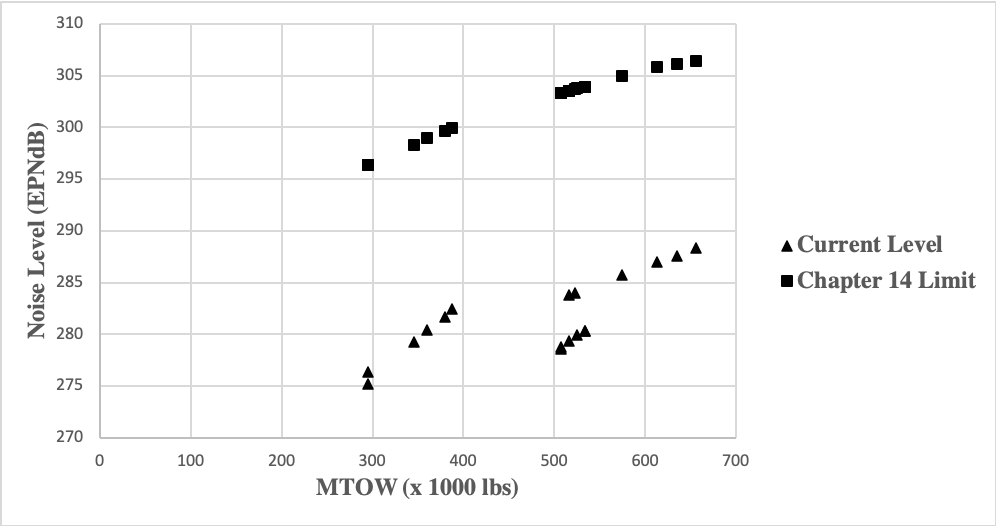
\includegraphics[width=\linewidth]{Photos/Noise_level.png}
    \caption{Noise Levels and Limits for Jet Aircraft}
    \label{fignoise}
\end{figure}

\subsection{Acoustic Estimation and Model Inaccuracies} 



In order to estimate the Sam Mk I's acoustic decibel value, multiple similar aircrafts with engines that were incorporated in the propulsion trade study were examined. Certification data was taken from the PW 4000, the RB Trent 7000, and the Sam Mk I's engine, the GE90-115B. Cumulative noise levels from these engines were retrieved from the EASA database \cite{easa}, along with their respective limits in accordance to Chapter 14. The aircraft's max take-off weights with the engines described above were then plotted against their respective EPNdBs in Figure \ref{fignoise}. The aircraft GE90-115B engine data that was extracted from EASA \cite{easa} was almost double that of the SAM Mk I's MTOW. To estimate the SAM Mk I's acoustic levels, the aircraft's weight was proportionally halved, which resulted in an approximate cumulative noise level of 275-279.3 EPNdB, well below the Chapter 14 limit of 296.5 for a 365,000 lb aircraft. Since the aircrafts taken in the acoustic similarity analysis contain two engines, just like the SAM Mk I, there is no need to account for additional engine noise. If there were a 3 EPnDB buffer to account for additional airframe noise, the SAM Mk I would still be well below the required limit. Although the estimated noise levels are well below the limit outlined in Chapter 14, it is worth noting that this is not the guaranteed acoustic performance for the SAM Mk I. This model is simply a preliminary estimation of the noise levels. The SAM Mk I was proportionally halved from ohter aircraft with the GE90-115B engine, but there could have been slight EPNdB differences in doing so, and furthermore, exact fuselage and wing noise levels were not taken into account. Despite this, however, the difference the above parameters would create for this aircraft's noise levels would be small, and still not close to the noise limit required for the SAM Mk I. 

There are multiple noise reduction techniques applied to the Sam Mk I. The aircraft incorporates an engine with a high bypass ratio, which allows for less noise to be emitted from the thrust of engine. Porous concepts are also another technique that can be incorporated in the Sam Mk I. NASA coordinated studies on experimental landing gear with fairings that are porous along their front and sound absorbing foam on the landing gear cavities, which resulted in overall reduction of airframe noise \cite{noise_reduction}. Although not present on current aircraft, when the Sam Mk I goes into production in 10 years, these landing gear techniques will be included, leading to an even further reduction of noise. 